\documentclass[hidelinks]{article}

%%%%%%%%%%%%%%%%%%%%%%%%%%%%%%%%%%%%%%%%%%%%%%%%%%%%%%%%%%%%%%%
% START CUSTOM INCLUDES & DEFINITIONS
%%%%%%%%%%%%%%%%%%%%%%%%%%%%%%%%%%%%%%%%%%%%%%%%%%%%%%%%%%%%%%%
\usepackage{amsmath,amssymb,amsfonts,amsthm}
%\usepackage{parskip} %noident everywhere
\usepackage{mathtools}
\usepackage{subcaption}
\usepackage{overpic}
\usepackage{mymath}
\usepackage{nth}
\usepackage{caption}
\usepackage{todonotes}
\usepackage{fullpage}
\usepackage{arydshln} % dashed line in array
\usepackage{MnSymbol} % anti-diag dots
%\usepackage{showlabels} % show equation and figure labels
\usepackage{subcaption}
\usepackage{varwidth, tikz}
\usetikzlibrary{shapes, arrows, shapes.misc, arrows.meta, positioning, matrix, calc, fit, fadings, patterns}
\usetikzlibrary{calc,patterns,decorations.pathmorphing,decorations.markings,arrows, arrows.meta}
\usepackage[export]{adjustbox}
\usepackage{placeins}
\setlength{\parindent}{0pt} 
\usepackage{tabto}

\newtheorem{lemma}{Lemma}
\newtheorem{definition}{Definition}
\newtheorem{theorem}{Theorem}
\newtheorem{corollary}{Corollary}
\newtheorem{proposition}{Proposition}
\newtheorem{assumption}{Assumption}

%%%%%%%%%%%%%%%%%%%%%%%%%%%%%%%%%%%%%%%%%%%%%%%%%%%%%%%%%%%%%%%
%%% ALG STUFF
%%%%%%%%%%%%%%%%%%%%%%%%%%%%%%%%%%%%%%%%%%%%%%%%%%%%%%%%%%%%%%%
\usepackage{algorithm}
\usepackage{algorithmic}
\newcommand{\algorithmicbreak}{\textbf{break}}
\newcommand{\Break}{\State \algorithmicbreak}
\renewcommand{\algorithmicrequire}{\textbf{Input:}}
\renewcommand{\algorithmicensure}{\textbf{Output:}}
\makeatletter
\newcommand{\algrule}[1][.2pt]{{\color{black!10!white}{\par\vskip.1\baselineskip\hrule height #1\par\vskip.1\baselineskip}}}
\makeatother
%\usepackage[linesnumbered,ruled,vlined]{algorithm2e}
%%%%%%%%%%%%%%%%%%%%%%%%%%%%%%%%%%%%%%%%%%%%%%%%%%%%%%%%%%%%%%%
% END CUSTOM INCLUDES & DEFINITIONS
%%%%%%%%%%%%%%%%%%%%%%%%%%%%%%%%%%%%%%%%%%%%%%%%%%%%%%%%%%%%%%%

\pdfobjcompresslevel=0

\title{Fast Gradient Method and Dykstra's Alternating Projection}
\author{Idris Kempf}
\begin{document}
\maketitle
\section{Problem Statement}
Consider the state-space representation of a linear system in discrete time,
\begin{subequations}
\begin{align}\label{eq:statespace}
{x}_{k+1}&={A}{x}_{k}+{B}{u}_{k},\quad u_k\in\mathcal{U}({u}_{k\sm 1}),\\
{y}_{k}&={C}{x}_{k}+{d}_{k},
\end{align}
\end{subequations}
where $\inRv{{y}_k}{n_y}$ are the outputs at time $t=k T_s$ and $\inRv{{x}_k}{n_x}$ are the states. The inputs $\inRv{{u}_k}{n_u}$ are subjected to amplitude and slew-rate constraints that can be modeled as $\mathcal{U}({u}_{k\sm 1})\eqdef\mathcal{A}\cap\mathcal{R}({u}_{k\sm 1})$, where ${u}_{k\sm 1}$ is the input applied at time $t=(k-1) T_s$ and $\mathcal{A}$ and $\mathcal{R}({u}_{k\sm 1})$ are the amplitude and slew-rate constraint sets:
\begin{subequations}\label{eq:constraints}
\begin{align}
\mathcal{A}&\eqdef\set{{u}_{k}\in\R^{n_u}}{-\alpha \leq {u}_{k} \leq \alpha},\\
\mathcal{R}({u}_{k\sm 1})&\eqdef\set{{u}_{k}\in\R^{n_u}}{-\rho \leq {u}_{k}\sm {u}_{k\sm 1} \leq \rho}.
\end{align}
\end{subequations}

The condensed model predictive control problem for~\eqref{eq:statespace} is
\begin{align}\label{eq:qpshort}
\min_{{u}} \frac{1}{2}\trans{{u}}{J}{u}+\trans{{q}({\hat{x}}_k, {\hat{d}}_k)}{u}\quad\text{s.t.}\quad{u}\in\mathcal{S}({u}_{\sm 1}),
\end{align}
where ${u}\eqdef({u}_0^\Tr,\dots,{u}_{N\sm 1}^\Tr)^\Tr\!\in\!\R^{Nn_u}\!$, $N$ the horizon, $f(u)\eqdef\frac{1}{2}\trans{{u}}{J}{u}+\trans{{q}({\hat{x}}_k, {\hat{d}}_k)}{u}$ the objective function and $\inR{{J}=\trans{{J}}}{Nn_u}{Nn_u}$ the Hessian. The vector ${q}({\hat{x}}_k, {\hat{d}}_k)$ is an affine function of the observer output ${\hat{x}}_k$ and ${\hat{d}}_k$. The closed convex set $\mathcal{S}({u}_{\sm 1})$ is defined as
\begin{align}\label{eq:set}
\mathcal{S}({u}_{\sm 1})\eqdef\mathcal{U}({u}_{\sm 1})\times\dots\times\,\mathcal{U}({u}_{N\sm 2}),
\end{align}
and depends on the input ${u}_{\sm 1}$ applied at time $t-1$. The following assumptions on problem~\eqref{eq:qpshort} are made throughout the paper: 
\newtheorem*{ass1}{Assumption I.a}
\begin{ass1}[Strong convexity]
It holds that $0\prec \lambda_\text{min}I\preceq J\preceq\lambda_\text{max}I$, where $\lambda_\text{min}$ and $\lambda_\text{max}$ are the minimum and maximum eigenvalues of $J$. 
\end{ass1}
\newtheorem*{ass2}{Assumption I.b}
\begin{ass2}[Bounded inputs]
The set $\mathcal{S}$ is bounded, so that $\abs{\mathcal{S}}\eqdef \max_{x,y\in\mathcal{S}}\,\twonorm{x-y}<\infty$.
\end{ass2}

To solve problem~\eqref{eq:qpshort}, we are using the fast gradient method shown in Algorithm~\ref{alg:fgm}. The present variant of the fast gradient method is applicable to strongly convex functions for ill-conditioned Hessians~\cite[Ch. 2.2.4]{OPTIMNESTEROV}. The fast gradient method requires the Eucledian projection $\mathcal{P}_{\mathcal{S}}$ onto $\mathcal{S}$, and no simple formula exists for $N>1$. Here, we are replacing the exact projection $\mathcal{P}_{\mathcal{S}}$ with Dykstra's alternating projection algorithm, $\mathcal{D}_{\mathcal{S}}$. Dykstra's method is an interative algorithm that yields the exact projection if the algorithm is run for an infinite number of iterations. For $M$ iterations, $\mathcal{D}_\mathcal{S}(z)\not\in\mathcal{S}$ in general\footnote{For example, consider the projection onto a corner (or edge) of two intersecting hyperplanes.} and the method yields a projection error that can be quantified as shown in the following assumption.
\newtheorem*{ass3}{Assumption II}
\begin{ass3}[Approximate projection]
Dykstra's method $\mathcal{D}_{\mathcal{S}}$ returns a point $\mathcal{D}_{\mathcal{S}}(z)$ that satisfies
\begin{align}
\twonorm{\mathcal{D}_{\mathcal{S}}(z) - \mathcal{P}_{\mathcal{S}}(z)} \leq \delta (z,M,\mathcal{S}),
\end{align}
where the upper bound $\delta (z,M,\mathcal{S})>0$ depends on the maximum number of iterations $M$ of Dykstra's method.
\end{ass3}
The aim of this paper is to
\begin{enumerate}
\item Characterize $\delta (z,M,\mathcal{S})$ for $\mathcal{S}$ and $z\in\mathcal{Z}$, where $\mathcal{Z}=\mathcal{Z}(J,q,u_{\sm 1})$ is to be defined.
\item Analyze the converge of Algorithm~\ref{alg:fgm} for fixed $M$.
\end{enumerate}
The ideal result would be to obtain a formula that relates $M$ and $\epsilon$, where $\epsilon$ represents an upper bound on the solution accuracy of the modified fast gradient method. 
%
\begin{algorithm}[H]
 \caption{Fast gradient method: Constant step scheme III with parameter~\cite[Ch. 2.2.4]{OPTIMNESTEROV}.}\label{alg:fgm}
 \begin{algorithmic}[1]
    \REQUIRE ${u}_{k\sm 1}\rightarrow v_0$
    \ENSURE ${u}_k\leftarrow p_M$
    \STATE Set $p_0=0$
	\FOR{$i = 0$ to $M-1$}
  	  \STATE ${z}_{i+1} = (I - {J}\inv{\lambda}_{max}){v}_i - {q} \inv{\lambda}_{max}$
  	  \STATE ${p}_{i+1} = \mathcal{P}_{\mathcal{S}}({z}_{i+1})$
  	  \STATE ${v}_{i+1} = (1+\beta){p}_{i+1} - \beta {p}_i$
	\ENDFOR
 \end{algorithmic}
\end{algorithm}
%
\section{Fast Gradient Method}
A convergence analysis of Algorithm~\ref{alg:fgm2} is presented in~\cite{FGMPROJECTION} with $\mathcal{P}_{\mathcal{S}}$ replaced by $\mathcal{D}_{\mathcal{S}}$ satsifying
\begin{align}
\twonorm{\mathcal{D}_{\mathcal{S}}(z) - \mathcal{P}_{\mathcal{S}}(z)} \leq \delta,
\end{align}
where $\delta>0$ is an arbitrary constant. Note that Algorithm~\ref{alg:fgm} is obtained from Algorithm~\ref{alg:fgm2} by setting $\alpha_0^2=\lambda_\text{max}/\lambda_\text{min}$. The authors prove that if
\begin{align}
\delta \leq \frac{\epsilon\lambda_\text{max}^{1/2}}{120\lambda_\text{min}^{3/2}\abs{\mathcal{S}}},
\end{align}
then at most $K$ iterations of Algorithm~\ref{alg:fgm2},
\begin{align}
K=\left\lceil\sqrt{\frac{\lambda_\text{max}}{\lambda_\text{min}}}\log\left(
\frac{3\lambda_\text{min}r_1^2+6(f(\mathcal{P}_\mathcal{S}(z_1))-f^\star)}{\epsilon}
\right)\right\rceil,
\end{align}
are required to obtain a solution $p_K$ that satisfies
\begin{align}
&\text{dist}_\mathcal{S}(p_K)\leq\epsilon,& f(p_K)-f^\star\leq\epsilon,
\end{align}
where $\text{dist}_\mathcal{S}(y)\eqdef\min_{x\in\mathcal{S}}\twonorm{x-y}$, $f^\star=f(u^\star)$ is the minimum of~\eqref{eq:qpshort} and $r_k\eqdef\twonorm{p_k-u^\star}$.
%
\begin{algorithm}[H]
 \caption{Fast gradient method: Constant step scheme III~\cite[Ch. 2.2.4]{OPTIMNESTEROV} with approximate projection.} \label{alg:fgm2}
 \begin{algorithmic}[1]
    \REQUIRE ${u}_{k\sm 1}\rightarrow v_0$
    \ENSURE ${u}_k\leftarrow p_M$
    \STATE Set $p_0=0$
	\FOR{$i = 0$ to $M-1$}
  	  \STATE ${z}_{i+1} = (I - {J}\inv{\lambda}_{max}){v}_i - {q} \inv{\lambda}_{max}$
  	  \STATE ${p}_{i+1} = \mathcal{D}_{\mathcal{S}}({z}_{i+1})$
  	  \STATE $\alpha_{i+1}^2=(1-\alpha_{i+1})\alpha_i^2+\alpha_{i+1}\lambda_\text{max}/\lambda_\text{min}$
  	  \STATE $\beta_{i+1}=\alpha_i(1-\alpha_i)/(\alpha_i^2+\alpha_{i+1})$
  	  \STATE ${v}_{i+1} = (1+\beta_{i+1}){p}_{i+1} - \beta_{i+1} {p}_i$
	\ENDFOR
 \end{algorithmic}
\end{algorithm}
%
\section{Dykstra's Alternating Projection}
Given $r$ convex sets $\mathcal{H}_1,\dots,\mathcal{H}_r$, Dykstra's alternating projection algorithm~\cite{DYKSTRA,Han1988} finds the orthogonal projection $x^\star$ of $x$ onto $\mathcal{H}\eqdef{\bigcap}_{i=1}^r \mathcal{H}_i$ by iterating over
\begin{align}\label{eq:dykstra}
&x_n=\mathcal{P}_{\mathcal{H}_{[n]}}\left(x_{n-1}+e_{n-r}\right),
&e_n=x_{n-1}+e_{n-r}-x_n,
\end{align}
where $[n]= \set{n+mr}{m\in\mathbb{Z}}\cap\lbrace 1,\dots,r\rbrace$,  $x_0=x$ and $e_i=0$ when $i\leq 0$. The Boyle-Dykstra theorem~\cite{DYKSTRA} implies that $\lim_{n\rightarrow\infty}\anynorm{x_n-\mathcal{P}_\mathcal{H}(x)}=0$. For a finite number of iterations, there is no guarantee that $x_n\in\mathcal{H}$. 

Here, we assume that $\mathcal{H}$ is a polyhedron and the $\mathcal{H}_i$ are halfspaces given by
\begin{align}\label{eq:sets_i}
\mathcal{H}_i\eqdef\set{x}{\iprod{x}{f_i} \leq c_i},
\end{align}
where $\anynorm{f_i}=1$. In addition, define
\begin{align}\label{eq:sets_i2}
H_i\eqdef\set{x}{\iprod{x}{f_i} = c_i},
\end{align}
so that $\text{int}\,\mathcal{H}_i\eqdef\mathcal{H}_i\backslash H_i$. The projections onto $H_i$ and $\mathcal{H}_i$ are given by
\begin{align}
&\mathcal{P}_{H_i}(x)=x-\left(\iprod{x}{f_i} - c_i\right)f_i,
&\mathcal{P}_{\mathcal{H}_i}(x)=\begin{cases}
x & \text{if } x\in\mathcal{H}_i\\
\mathcal{P}_{H_i}(x) & \text{if } x\not\in\mathcal{H}_i\,.
\end{cases}
\end{align}
For this particular choice of sets, $e_n = k_n f_{[n]}$ with $k_n=\text{dist}_{\mathcal{H}_{[n]}}(x_{n-1}+e_{n-r})$, i.e. the auxiliary vector is either $0$ or parallel to $f_{[n]}$. 

The convergence of Dykstra's method has been analyzed in~\cite{DYKSTRAPOLY2,DYKSTRAPOLY}, where it has been shown that the convergence is linear. In~\cite{DYKSTRAPOLY}, the proof is based on partitioning the set $\lbrace 1,\dots,r\rbrace$ into
\begin{align}
&A=\set{i\in\lbrace 1,\dots,r\rbrace}{x_\infty\in H_i},
&B=\lbrace 1,\dots,r\rbrace\backslash A=\set{i\in\lbrace 1,\dots,r\rbrace}{x_\infty\in\text{int}\,\mathcal{H}_i},
\end{align}
where $x_\infty=\lim_{n\rightarrow\infty}x_n$. It can be shown that there exists a number $N_1$ such that whenever
\begin{align}
[n]\in B,\quad n\geq N_1\quad\Rightarrow\quad x_n=x_{n-1},\quad e_n=0,
\end{align}
i.e. the half-spaces in $B$ become ``inactive''. Furthermore, there exists $N_2\geq N_1$ such that whenever $n\geq N_2$, it holds that
\begin{align}
\twonorm{x_{n+r}-x_\infty}\leq\alpha_{[n]}\twonorm{x_n-x_\infty},
\end{align}
where $0\leq\alpha_{[n]}<1$. With these ingredients, the following result is obtained:
\begin{theorem}
There exist constants $0\leq c < 1$ and $\rho > 0$ such that
\begin{align*}
\anynorm{x_n -x_\infty} \leq \rho c^n.
\end{align*}
\end{theorem}
The factor $c$ can be estimated from the smallest $\alpha_{[n]}$, which is characterized by the angle between certain subspaces (subspaces formed by the ``active'' halfspaces). The factor $\alpha_{[n]}$ can be upper-bounded by considering the ``worst'' angles in the polyhedron.

The constant $\rho$, however, depends on a number $N_3\geq N_2$ and on $x$. It is unclear how to obtain that constant $\rho$. In fact, the authors of~\cite{DYKSTRAPERKINS} and~\cite{XUPOLY} emphasize that $\rho$ cannot be computed in advance, and that the inability to compute a bound on the projection error makes the application of Dykstra's method difficult. The authors of~\cite{DYKSTRAPERKINS} proposed a combined Dysktra-conjugate-gradient method that allows for computing an upper bound on $\anynorm{x_n -x_\infty}$. The authors of~\cite{XUPOLY} proposed an alternative algorithm called \emph{successive approximate algorithm}, which promises fast convergence, conditioned on knowing a point $x\in\mathcal{H}$ in advance.
%
\section{Stalling}
%
In~\cite{DYKSTRASTALLING}, the behavior of Dykstra's method is analalyzed for two sets. The authors give conditions on Dykstra's algorithm for (1) finite convergence, (2) infinite convergence and (3) stalling followed by infinite convergence. 

A specific example is given for the case that the set is given by the intersection of a line with a unit box in $\R^2$ ($\mathcal{H}$ is a polyhedron). It can be shown that cases 1--3 depend on the starting point $x_0$, and one can determine the 3 regions shown in Figure~\ref{fig:region} that yield that yield the different convergence behavior. Convergence case 1 is obtained when starting in the green region, case 2 when starting in the blue region and case 3 when starting in the red region.

To understand the stalling effect, consider Figure~\ref{fig:stalling}, which shows the first iterations of Dykstra's algorithm with starting point in the red region. Note that the outcome of Dykstra's algorithm depends on the order of the sets $\mathcal{H}_i,\dots,\mathcal{H}_r$. In Figure~\ref{fig:stalling}, the algorithm starts by projecting onto the line and then onto the box. It can be seen that for the first 6 iterations\footnote{By one iteration we mean one cycle of $r$ projections here.}, Dykstra's algorithm returns the top left corner of the box (``stalling''). The author's also determine the exact number of iterations required to break-free from the red region, and show that if the starting point is arbitrarily far to the left, the algorithm will need an arbitrarily large iteration number for breaking-free from the red region.
%
\begin{figure}
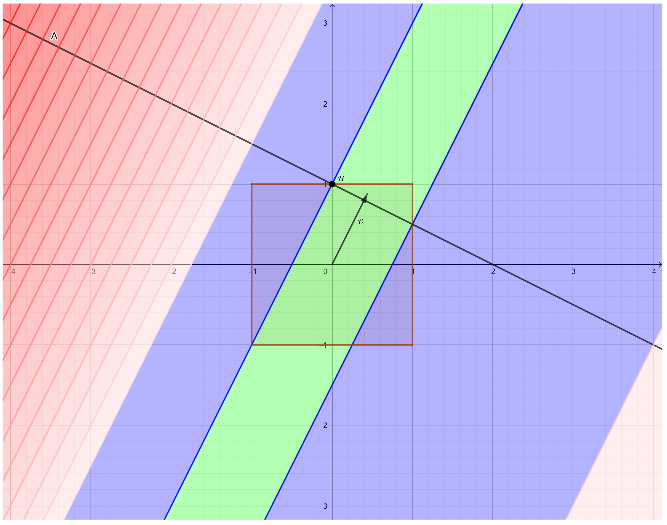
\includegraphics[width=0.6\linewidth]{regions.png}\caption{Line-box example with different regions that yield different convergence properties.}\label{fig:region}
\end{figure}
%
%
\begin{figure}
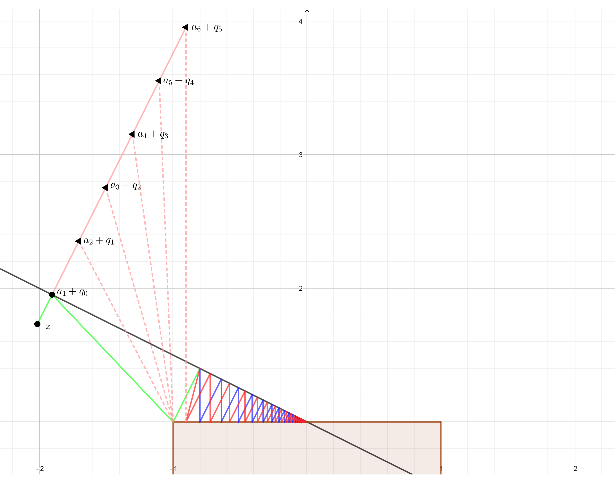
\includegraphics[width=0.6\linewidth]{stalling.png}\caption{Stalling for the line-box example when $x_0$ is in the red region.}\label{fig:stalling}
\end{figure}
%
\section{Thoughts}
%
In theory, the formulae presented in these notes would allow for determining the solution accuracy of the fast gradient method if both the fast gradient method and Dykstra's algorithm are run for a fixed number of iterations. However, because the error bound for Dykstra's method cannot easily be computed in advance\footnote{For an arbitrary polyhedral set. It can be computed for e.g. 2 sets.}, the formulae cannot be applied.

The results on the fast gradient method are surprising. I do not understand how one can obtain a solution with $\epsilon$ accuracy if the approximate projection returns the unchanged vector, for example. However, it does seem that the proof requires the projection error to be bounded by $\delta$ (regardless of the starting point), in which case the former example does not work.

It seems obvious that there is a connection between the stalling and the inability to compute the error bound in advance. E.g. consider the stalling situation from last section (Figure~\ref{fig:stalling}). It is my impression that the constant $c$ in the Dykstra error bound could be computed after the stalling period (note that $N_2$ is reached after the stalling period -- one needs to model the box via halfplanes, in which case we enter the interior of the halfplane defining the left side of the box).

Questions:
\begin{itemize}
\item Can Dysktra's method be modified to escape the stalling region in a finite number of iterations?\\
It does seem that introducing $e_n=e_{n-r}+\beta_n (x_{n-1}-x_n)$ improves things.
\item Can Dysktra's method be accelerated after escaping the stalling region?\\
\item Can we replace Dykstra's method by the \emph{successive approximate algorithm}~\cite{XUPOLY}?\\
The previously computed input is always feasible.
\item Can we modify Dykstra's method such that it becomes independent of the set ordering?\\
This should be possible to formulate mathematically. However, it does make sense to obtain different ``trajectories''. The convergence properties should be independent of set ordering.
\item Is there some heuristic for the set ordering?\\
I have tried a few without success.
\end{itemize}
%
\section{Acceleration for Dykstra's Method}
%
Consider introducing the step size parapemeter $\beta_n\geq 0$:
\begin{align}\label{eq:dykstramodif}
&x_n=\mathcal{P}_{\mathcal{H}_{[n]}}\left(x_{n-1}+e_{n-r}\right),
&e_n=e_{n-r}+\beta_n(x_{n-1}-x_n).
\end{align}
For $\beta_n=0$, we obtain Von Neumann's \emph{Alternating Projection Method} and for $\beta_n=1$, we obtain Dykstra's method~\eqref{eq:dykstra}. We proceed by characterizing the term $e_n$.
\begin{lemma}
It holds that $e_n=y_n f_{[n]}$, where
\begin{align*}
y_n = (1-\beta_n)y_{n-r} +k_n,
\end{align*}
and $k_n=\text{dist}_{\mathcal{H}_{[n]}}(x_{n-1}+e_{n-r})$.
\end{lemma}
\begin{proof}
Suppose that $x_{n-1}+e_{n-r}\in\inter\mathcal{H}_{[n]}$. Then, $x_n=x_{n-1}+e_{n-r}$ and
\begin{align*}
e_n=(1-\beta_n)e_{n-r}.
\end{align*}
Suppose that $x_{n-1}+e_{n-r}\not\in\inter\mathcal{H}_{[n]}$. Then, $x_n=x_{n-1}+e_{n-r}-\left(\iprod{x_{n-1}+e_{n-r}}{f_{[n]}} - c_i\right)f_{[n]}$ and
\begin{align*}
e_n=(1-\beta_n)e_{n-r}+k_nf_{[n]}.
\end{align*}
Note that $e_n=0$ for $n\leq 0$. By induction, $e_n$ is always parallel to $f_{[n]}$ or zero. Substituting $e_n=y_nf_{[n]}$ yields
\begin{align*}
y_n=(1-\beta_n)y_{n-r}+k_n.
\end{align*} 
\end{proof}

\bibliographystyle{plain}
\bibliography{master_bib_abbrev}
\end{document}